Das Ergebnis des Hörversuchs ist in Abbildung ~\ref{fig:versuch} zu sehen. Es wurden insgesamt 6 Personen mit geschultem Gehör befragt.

\begin{figure}[!ht]
  \centering
  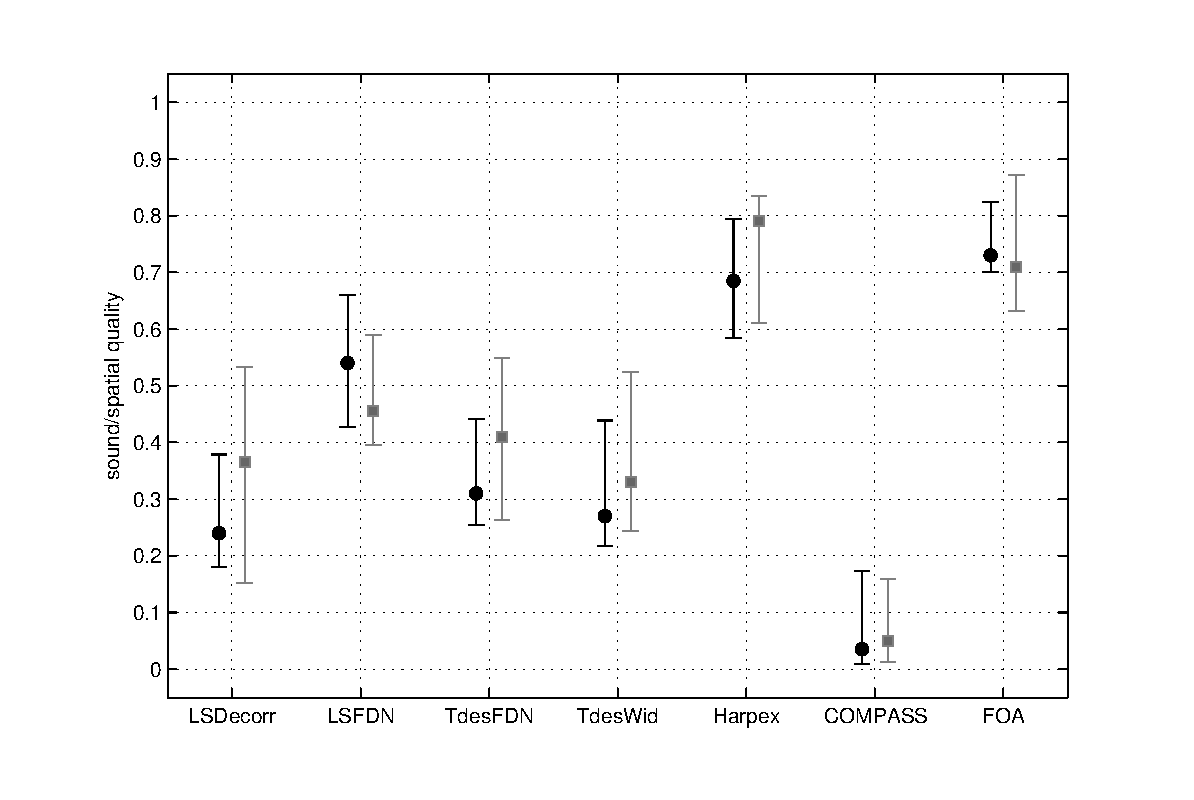
\includegraphics[width=1\textwidth]{ergebnis/plots/result.eps}
  \caption{Ergebnis des Hörversuchs, Median mit 95\% Konfidenzintervalle (Klangqualität in schwarz und räumliche Qualität in grau)}
  \label{fig:versuch}
\end{figure}

Die Bewertungen erfolgten nach zwei Kriterien:

\begin{itemize}
  \item Klangqualität: \textit{sehr gut} (1) bis \textit{sehr schlecht} (0)
  \item räumliche Qualität: \textit{realistisch} (1) bis \textit{synthetisch} (0)
\end{itemize}

Die Bewertungen nach den zwei gewählten Kriterien weisen eine hohe Korrelation auf. Dies deutet entweder auf eine tatsächliche Korrelation der Algorithmen von Klangqualität und räumlicher Wiedergabequalität hin, oder die Fragestellung zielt nicht auf genügend unterschiedliche Aspekte der Testsignale ab. Dabei können stärkere Artefakte als Verminderung der räumlichen Qualität des Algorithmus gedeutet werden.

Die gute Bewertung des Referenzsignals (FOA: first order ambisonics) ist ein überraschendes Ergebnis dieses Hörversuchs. Aus der Theorie ist zu erwarten, dass durch die Upmixing-Verfahren eine Verbesserung der Bewertungen eintritt. Dies kann wieder mit den Fragestellungen erklärt werden. Die Upmixing-Verfahren schärfen den gerichteten Signalanteil und ermöglichen eine Erhöhung der Diffusität des diffusen Anteils. Die Fragestellungen zielten jedoch auf Klangqualität und räumliche Qualität ab. Da FOA als Referenzsignal als Einziges unbearbeitet ist, ist auch zu erwarten, dass die Bewertung nach möglichen hörbaren Artefakten (Klangqualität) am besten ausfällt. Weiters kann argumentiert werden, dass eine künstliche Dekorrelation des Diffusanteils synthetischer wahrgenommen wird, als das originale aufgenommene Diffussignal des Aufnahmeraumes, obwohl FOA die räumliche Wiedergabequalität einschränkt.
Nach unseren Kriterien schneidet HARPEX als bester Upmixing-Algorithmus und COMPASS klar als schlechtester.

Die Bewertungen der verschiedenen DirAC Implementierungen liegen dazwischen und sind nicht statistisch signifikant unterschiedlich. Tendentiell ist LSFDN (DirAC dekodiert auf die physische Lautsprecheranordnung mit FDN zur Synthese des Diffussignals) als bester DirAC-Algorithmus bewertet worden.
Ein interessantes Ergebnis ist, dass LSFDN besser bewertet wurde, als LSDecorr (originale Diffussignalsynthese nach \cite{pulkki}). Der Unterschied der Klangqualität dieser zwei Algorithmen ist statistisch signifikant.
